% PREAMBLE -- START

\documentclass[12pt,dvipsnames]{article}
\usepackage{amsmath,epsfig,subfigure,fancybox}
\usepackage{amsfonts,amssymb,amsthm,xparse}
\usepackage{rotating}
\usepackage{times}
\usepackage{bbm}
\usepackage{bm}
\usepackage{verbatim}
\usepackage{mathrsfs,wrapfig}
\usepackage{smartdiagram}
%\usepackage{physics}

\oddsidemargin .25in
\evensidemargin .25in  
\textwidth 6in
\topmargin -0.4in      
\textheight 8.75in

% New commands to make life easy

%
% short cuts
%

\newcommand{\eref}[1]{(\ref{#1})}
\newcommand{\fref}[1]{Fig.~\ref{#1}}
\newcommand{\tref}[1]{Table~\ref{#1}}
\newcommand{\sref}[1]{Section~\ref{#1}}
\newcommand{\vm}[1]{\mathbf{#1}}
\newcommand{\vx}{\vm{x}}
\newcommand{\bsym}[1]{\boldsymbol{#1}}
\newcommand{\abs}[1]{{\lvert#1\rvert}}
\newcommand{\norm}[1]{{\lVert#1\rVert}}
\newcommand{\inner}[2]{(#1,#2)}
\renewcommand{\mathbbm}[1]{\vm{#1}}

\newcommand{\incolor}[1]{\Red{#1}}

%\usepackage{hyperref}
\usepackage{url,color,colordvi}
\graphicspath{ {./figures/} }

% PREAMBLE -- END

\begin{document}

\title{Radial Density Functional Theory}
\author{Subhajit Banerjee}
\date{\today}
\maketitle

\begin{abstract}
The formulation and implementation of radial Density Functional 
Theory is presented.  
\end{abstract}

\section{Strong form}
Consider the case of an isolated atom. Let this atomic system consists of 
$N$ electrons. In an uncharged atom, the atomic number $Z$ is also 
equal to $N$. In the paradigm of many-boy quantum  
mechanics applied to such atomic systems one is interested determining the 
single-particle (electronic) \emph{wavefunctions} (\emph{orbitals}) $\{ \psi_i(x_i) \}$. 
For spherically symmetric potential, as is the case for an isolated atom, the 
wavefunctions are often expressed as $\psi_{n \ell m} (\vx)$ where $n$ is the principal quantum number, 
$\ell$ is the orbital angular momentum quantum number, and $m$ is the magnetic quantum number. 
It can further be simplified (separation of variables):
$$\psi_{n \ell m} (\vx) \equiv \psi_{n \ell m} (r, \theta, \phi) = R_{n \ell}(r) Y_{\ell m}(\theta, \phi)$$
where $Y_{\ell m}(\theta, \phi)$ are the \emph{spherical harmonics} and $R_{n \ell}(r)$ satisfies the 
\emph{radial Schr{\"o}dinger equation}:
\begin{equation}	\label{radsch}
\Big( -\frac{1}{2} r^2 R^\prime_{n \ell}(r) \Big)^\prime + \Big( r^2 V(r) + \frac{1}{2} \ell (\ell + 1) \Big ) R_{n \ell}(r) = 
\varepsilon_{n \ell} r^2 R_{n \ell} (r)
\end{equation}
where $(\cdot)^\prime \equiv \dfrac{d(\cdot)}{dr}$.
\noindent
In \emph{Radial Density Functional Theory} the \emph {radial Kohn-Sham equation} is solved in a \emph{self consistent} manner. 
The radial Kohn-Sham equation, in spirit, is of similar form as eq.~\eqref{radsch} with the potential $V(r)$ 
being replaced by $\hat{V}_{\rm{eff}}[\rho_e(r)]$ where $\rho_e$ is the \emph{electronic density}. 
Hence, eq.~\eqref{radsch} can be rewritten as:
\begin{equation}	\label{radks}
\Big( -\frac{1}{2} r^2 R^\prime_{n \ell}[\rho_e(r)] \Big)^\prime + \Big( r^2 \hat{V}_{\rm{eff}}[\rho_e(r)] + \frac{1}{2} \ell (\ell + 1) \Big ) R_{n \ell}(r)[\rho_e(r)] = 
\varepsilon_{n \ell}[\rho_e(r)] r^2 R_{n \ell}[\rho_e(r)]
\end{equation}
where 
\begin{equation} \label{veff}
\hat{V}_{\rm{eff}}[\rho_e(r)] = V_H[\rho_e(r)] + V_{xc}[\rho_e(r)] + V_n(r).
\end{equation}
In eq.~\eqref{veff} $V_{xc}$ is known as the \emph{exchange-correlation} functional, 
$V_n(r) = -\frac{Z}{r}$ is the potential arising from the coulomb attraction of nucleus and $V_H$ is 
the \emph{Hartree potential}. The Hartree potential is governed by the \emph{radial Poisson 
equation}:
\begin{equation} \label{radpois}
\frac{1}{r^2} \Big( r^2 V^\prime_H(r) \Big)^\prime = V^{\prime \prime}_H (r) + \frac{2}{r} V^\prime_H(r) = -4 \pi \rho_e(r).
\end{equation}

\noindent
Note that eq.~\eqref{radks} is a nonlinear ordinary differential equation. This can further be 
elucidated by expressing $\rho_e(r)$ in terms of $R_{n \ell}$ which is done next. 
%
\subsection{Electron Density $\rho_e$} \label{sec:nonlin}
The electronic density $\rho_e$ is calculated by adding all $(n, \ell, m)$ states together, counting each one
twice (for spin up $\uparrow$ and spin down $\downarrow$) such that
\begin{align*}
\rho_e(r) & = 2 \sum\limits_{n \ell m} \vert \psi_{n \ell m} \vert^2 \\
& = 2 \sum\limits_{n \ell m}  R_{n \ell}^2 \vert Y_{\ell m} \vert^2\\
& = \Big( \sum\limits_{n \ell} R_{n \ell}^2 \Big) \Big(2 \sum\limits_m \vert Y_{\ell m} \vert^2 \Big) =  \frac{1}{4 \pi} \sum\limits_{n \ell} f_{n \ell} R_{n \ell}^2
\end{align*}
where the \emph{occupation numbers} $f_{n \ell}$ are defined as
\begin{equation}		\nonumber
f_{n \ell} = 2 \Big( 4 \pi \sum\limits_m \vert Y_{\ell m} \vert^2 \Big).
\end{equation}
Hence, we get the following circular dependency:\\
\begin{center}
\smartdiagram[flow diagram:horizontal]{$\rho_e$, $\hat{V}_{\rm{eff}}$, $R_{n \ell}$}
%\smartdiagram[circular diagram:clockwise]{$\rho_e$, $\hat{V}_{\rm{eff}}$, $R_{n \ell}$}
\end{center}
%
%
\section{Weak form}
The weak form (principle of virtual work) or equivalently the minimization 
of the potential energy functional is derived next. 
%
\subsection{Radial Kohn-Sham Equation}
We multiply eq.~\eqref{radks} by an arbitrary 
\emph{test or weighting function\/} $v(r)$ and integrate over the spherical volume 
of radius $a$ to obtain: 
\begin{multline*}
\int\limits_0^{\pi} \int\limits_0^{2 \pi} \int\limits_0^a \Big\{\Big( -\frac{1}{2} r^2 R^\prime_{n \ell}(r) \Big)^\prime + \Big( r^2 \hat{V}_{\rm{eff}}(r) + \frac{1}{2} \ell (\ell + 1) \Big ) 
R_{n \ell}(r) \Big\} v(r) r^2 \sin\theta \, \mathrm{d}r \mathrm{d}\theta \mathrm{d}\phi \\
= \varepsilon_{n \ell} \int\limits_0^{\pi} \int\limits_0^{2 \pi} \int\limits_0^a R_{n \ell} (r) v(r) r^2 \sin\theta \, \mathrm{d}r \mathrm{d}\theta \mathrm{d}\phi \qquad \forall v(r),
\end{multline*}
where $v$ is at least a piece-wise continuous function ($v \in C^0([0 \, \, a])$ will suffice).
Integrating over the angles gives $4 \pi$ which cancels from both sides, resulting in:
\begin{equation}	\label{wfinter}
\int\limits_0^a \Big\{\Big( -\frac{1}{2} r^2 R^\prime_{n \ell}(r) \Big)^\prime + \Big( r^2 \hat{V}_{\rm{eff}}(r) + \frac{1}{2} \ell (\ell + 1) \Big ) 
R_{n \ell}(r) \Big\} v(r) r^2 \mathrm{d}r  = \varepsilon_{n \ell} \int\limits_0^a R_{n \ell} (r) v(r) r^2 \mathrm{d}r.
\end{equation}
Applying integration by parts on the first-term of the left hand side of eq.~\eqref{wfinter}, we obtain, 
\begin{multline*}
\int\limits_{0}^a \Big\{ \frac{1}{2} R^\prime_{n \ell}(r) v^\prime(r) + \Big( \hat{V}_{\rm{eff}}(r) + \frac{1}{2}\ell(\ell + 1) \Big ) R_{n \ell}(r) v(r) \Big\} r^2 \, \mathrm{d} r 
- \frac{1}{2} \left[ r^2 R^\prime_{n \ell}(r) v(r) ]\right]_0^a \\ 
= \varepsilon_{n \ell} \int\limits_{0}^a R_{n \ell} (r) v(r) r^2 \, \mathrm{d} r.
\end{multline*}
The boundary term is zero at the origin ($r = 0$), so we get:
\begin{multline*}
\int\limits_{0}^a \Big\{ \frac{1}{2} R^\prime_{n \ell}(r) v^\prime(r) + \Big( \hat{V}_{\rm{eff}}(r) + \frac{1}{2}\ell(\ell + 1) \Big ) R_{n \ell}(r) v(r) \Big\} r^2 \, \mathrm{d} r 
- \frac{1}{2} a^2 R^\prime_{n \ell}(a) v(a) \\ 
= \varepsilon_{n \ell} \int\limits_{0}^a R_{n \ell} (r) v(r) r^2 \, \mathrm{d} r.
\end{multline*}
We usually want to have the boundary term $\frac{1}{2} a^2 R^\prime_{n \ell}(a) v(a)$ equal to zero. This is equivalent to either letting 
$R^\prime_{n \ell}(a) = 0$ (we prescribe the zero derivative of the $R_{n \ell}$ at $a$) or we set $v(a) = 0$ (which corresponds to zero 
Dirichlet condition for $R_{n \ell}$, i.e. setting $R_{n \ell}(a) = 0$).
In either of these situations, the last equation simplifies to: % $\lim\limits_{r \to 0} r^2 R^\prime_{n \ell}(r) = 0$
\begin{equation}	\nonumber
\int\limits_{0}^a \Big\{ \frac{1}{2} R^\prime_{n \ell}(r) v^\prime(r) + \Big( \hat{V}_{\rm{eff}}(r) + \frac{1}{2}\ell(\ell + 1) \Big ) R_{n \ell}(r) v(r) \Big\} r^2 \, \mathrm{d} r  
= \varepsilon_{n \ell} \int\limits_{0}^a R_{n \ell} (r) v(r) r^2 \, \mathrm{d} r.
\end{equation}
This point onwards we will only consider the case of $R_{n \ell}(0) = R_{n \ell}(a) = 0$, i.e., 
Dirichlet condition at both ends.

\noindent
Formally, the weak form is written as: find the \emph{trial function} (eigenfunction) 
$R_{n \ell}(r) \in {\cal S}$ and the eigenvalue $\varepsilon_{n \ell} \in \mathbb{R}$
such that
\begin{multline} \label{weakks}
\int\limits_{0}^a \Big\{ \frac{1}{2} R^\prime_{n \ell}(r) v^\prime(r) + \Big( \hat{V}_{\rm{eff}}(r) + \frac{1}{2}\ell(\ell + 1) \Big ) 
R_{n \ell}(r) v(r) \Big\} r^2 \, \mathrm{d} r  = \\
\varepsilon_{n \ell} \int\limits_{0}^a R_{n \ell} (r) v(r) r^2 \, \mathrm{d} r \qquad \forall v(r) \in {\cal V}
\end{multline}
where the trial and test function spaces, respectively, are
\begin{align*}
{\cal S} &= \{ R: R \in H^1([0 \, \, a]), \ R(0) = 0, \ R(a) = 0 \}, \\
{\cal V} &= \{ v: v \in H^1([0 \, \, a]), \ v(0) = 0, \ v(a) = 0 \},
\end{align*}
where $H^k([0 \, \, a])$ is the \emph{Sobolev space} that contains
functions that are square-integrable ($L^2([0 \, \, a])$) up to order $k$.
%
\subsection{Radial Poisson Equation}
To derive the weak form of radial Poisson equation, we proceed along the similar route as 
the last section. To this end, we first multiply eq.~\eqref{radpois} by an arbitrary 
test function $w(r)$ and integrate over the spherical volume 
of radius $a$ to obtain: 
\begin{equation*}
\int\limits_0^{\pi} \int\limits_0^{2 \pi} \int\limits_0^a \frac{1}{r^2} \Big( r^2 V^\prime_H(r) \Big)^\prime w(r) r^2 \sin\theta \, \mathrm{d}r \mathrm{d}\theta \mathrm{d}\phi = \\
 - 4 \pi \int\limits_0^{\pi} \int\limits_0^{2 \pi} \int\limits_0^a \rho_e(r) w(r) r^2 \sin\theta \, \mathrm{d}r \mathrm{d}\theta \mathrm{d}\phi \quad \forall w(r)
\end{equation*}
Next, after cancelling the $4 \pi $ arising from the integrals over the angles on both sides, and by 
applying integration by parts on the left hand side, we obtain
\begin{equation*}
\left[ r^2 V^\prime_H(r) w(r) \right]_0^a - \int\limits_0^a r^2 V^\prime_H(r) w^\prime(r) \mathrm{d}r = - 4 \pi \int\limits_0^a \rho_e(r) w(r) r^2 \mathrm{d}r
\end{equation*}
which, upon assuming $w(0) = w(a) = 0$ (or $w(0) = 0$ and $V^\prime_H(a) = 0$) simplifies to
\begin{equation*}
\int\limits_{0}^a V^\prime_H(r) w^\prime(r) r^2 \, \mathrm{d} r = 4 \pi \int\limits_{0}^a \rho_e(r) w(r) r^2 \, \mathrm{d} r.
\end{equation*}
Writing the last equation in more formal setting- the weak form statement of radial Poisson equation is: 
find the trial function $V_H(r) \in {\cal S}$ such that
\begin{equation} \label{weakpois}
\int\limits_{0}^a V^\prime_H(r) w^\prime(r) r^2 \, \mathrm{d} r = 4 \pi \int\limits_{0}^a \rho_e(r) w(r) r^2 \, \mathrm{d} r \qquad \forall w(r) \in {\cal V}
\end{equation}
where the trial and test function spaces are as defined previously.
%
\section{Trial and test approximations and discrete generalized eigenproblem}
\subsection{Radial Kohn-Sham Equation}
The spectral finite element (FE) approximation (trial function) can be written as 
(dropping the subscript $n, \ell$ for brevity)
\begin{equation}	\label{eq:fem}
R^h (r) = \sum_{j=1}^N \phi_j(r) R_j \in {\cal S}^h \subset {\cal S},
\end{equation}
where ${\cal S}^h$ is a finite-dimensional subspace of ${\cal S}$. In
addition, $\phi_j(r)$ are higher-order (spectral) finite element 
basis functions, and $R_j$ are the finite element degrees of freedom. 
The derivative of $R^h(r)$ is:
\begin{equation}\label{eq:dfem}
\bigl(R^h(r)\bigr)^\prime = \sum_{j=1}^N \phi_j^\prime (r) R_j.
\end{equation}

\noindent
In the interest of conciseness, I'll suppress the
dependence on $r$ for the functions that appear in the weak
form. On substituting $R^h$ and $(R^h)^\prime$
from~\eref{eq:fem} and~\eref{eq:dfem}, respectively, in eq.~\eqref{weakks}
 and letting $v^h$ be the test functions, we obtain:
\begin{multline*}
\int_0^a \Big\{ \sum_{j=1}^N \Big[ \frac{1}{2} (v^h)^\prime \phi_j^\prime + 
\Big( \hat{V}_{\rm{eff}}(r) + \frac{1}{2}\ell(\ell + 1) \Big ) v^h \phi_j \Big] R_j \Big\} r^2 \mathrm{d} r = \\
\varepsilon \int_0^a \sum_{j=1}^N v^h \phi_j R_j r^2 \mathrm{d} r \qquad \forall v^h \in {\cal V}^h.
\end{multline*}
Upon setting $v^h = \phi_i$ and denoting by $\vm{c} = \{R_1, \ldots, R_N\}$ leads to the \emph{ generalized eigenproblem}:
\begin{subequations}\label{eq:eigproblem}
\begin{align}
\vm{H}\vm{c} &= \varepsilon \vm{S} \vm{c}, \label{geneig}\\
\vm{H}_{ij} & = \int_0^a \Big[ \frac{1}{2} \phi_i^\prime \phi_j^\prime + 
\Big( \hat{V}_{\rm{eff}}(r) + \frac{1}{2}\ell(\ell + 1) \Big ) \phi_i \phi_j \Big] r^2 \mathrm{d} r \\
\vm{S}_{ij} & =  \int_0^a \phi_i \phi_j r^2 \mathrm{d} r.
\end{align}
\end{subequations} 
In the context of Schr\"odinger equation, $\vm{H}$ is known as the Hamiltonian matrix and 
$\vm{S}$ is the overlap matrix.
%
\subsection{Radial Poisson Equation}
Proceeding along the similar line as in the last section, the spectral finite element 
approximation (trial function) can be written as (dropping the subscript $H$ for brevity)
\begin{equation}	\label{eq:femV}
V^h (r) = \sum_{j=1}^N \phi_j(r) V_j \in {\cal S}^h \subset {\cal S}.
\end{equation}
In addition, $\phi_j(r)$ are higher-order (spectral) finite element 
basis functions, and $V_j$ are the finite element degrees of freedom. 
The derivative of $V^h(r)$ is:
\begin{equation}\label{eq:dfemV}
\bigl(V^h(r)\bigr)^\prime = \sum_{j=1}^N \phi_j^\prime (r) V_j.
\end{equation}
On substituting $V^h$ and $(V^h)^\prime$ from~\eref{eq:femV} and~\eref{eq:dfemV}, 
respectively, in eq.~\eqref{weakpois} and letting $w^h$ be the test functions, we obtain:
\begin{equation*}
\int_0^a \Big\{ \sum_{j=1}^N (w^h)^\prime \phi_j^\prime V_j \Big\} r^2 \mathrm{d} r = 4 \pi \int_0^a \rho_e w^h r^2 \mathrm{d} r \qquad \forall w^h \in {\cal V}^h.
\end{equation*}
Once again, setting $w^h = \phi_i$ and denoting by $\vm{u} = \{V_1, \ldots, V_N\}$ leads to the linear system:
\begin{subequations}\label{eq:linsys}
\begin{align}
\vm{K}\vm{u} &= \vm{b}, \\
\vm{K}_{ij} & = \int_0^a \phi_i^\prime \phi_j^\prime r^2 \mathrm{d} r \\
\vm{b}_i & = 4 \pi \int_0^a \rho_e \phi_i r^2 \mathrm{d} r.
\end{align}
\end{subequations}
%
\section{Self-Consistent Fields (SCF) Iterations}
Owing to the nonlinear nature of generalized eigenvalue problem in eq.~\eqref{geneig} as 
alluded in Section~\ref{sec:nonlin}, the problem is solved using the following self-consistent 
field technique:
\begin{center}
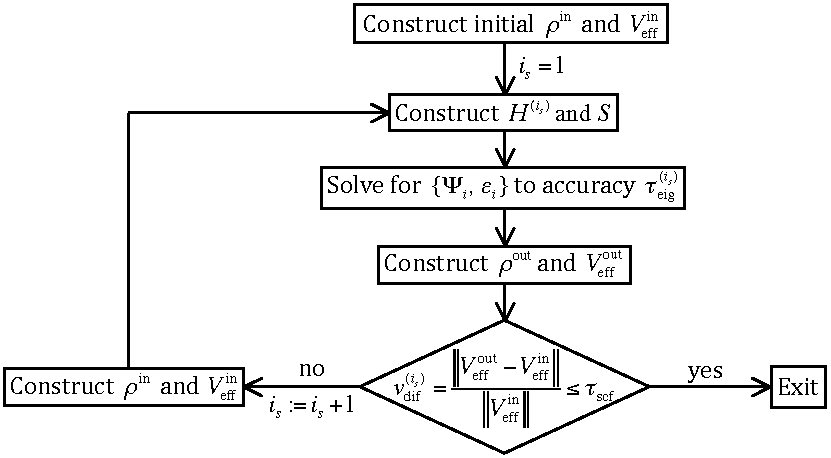
\includegraphics[width=1\textwidth]{scf.pdf}
%\caption{Schematic of the self-consistent field procedure.}
\end{center}

\end{document}
